% Section V: Results
% Every number traces to the POST-CORRECTION (commit 3a0f495) outputs in
% experiments/out/*.json; see PHASE_B_FINDINGS.md "Post-referee correction".
% Second-site SMBU numbers: smbu_rich_{record,eval}.json (production fit)
% and smbu_full_record.json (reference arm). Geometric accuracy vs the
% H3D reference mesh: geoacc_mar18.json.
% Stitched mass 0.980 / per-tile-renormalized 5.62: mass_oracle_mar18.json
% (persisted rerun of tests/test_eval_mass_oracle.py at its own seed).
% Synthetic slab check: change_synth_slab.json (persisted rerun of the
% tests/test_change_oracle.py synth_run fixture, seed 11).
% Remaining exception with no standalone JSON artifact: peak RSS 37.6 GB
% (PHASE_A_NOTES.md item 4, smbu_full run; flagged for PI).
% No invented numbers. Pre-fix stitched log-predictive values are void.

\section{Results}
\label{sec:results}

\subsection{Seam Handling: The Stitched Density at Parity with Hard
Deletion}
\label{sec:results:seams}

\looseness=-1 Table~\ref{tab:seam} reports the seam-rule comparison: held-out
log-predictive per point, stitched versus crop and Voronoi, under the
complement protocol of Sec.~\ref{sec:setup:protocols}. At production
capacity the rules are at \emph{parity}: stitched trails crop by
$0.02$--$0.03$~nats/point overall, with seam-subset differences from
$+0.01$ on March~2018 to
$-0.09$/$-0.14$ on the other epochs. At the reference arm the overall
gap is still only $-0.11$, but the seam bands show a real
$0.56$--$0.66$~nat stitched deficit (coarse components straddling
seams), which production capacity closes.

\looseness=-1 The SMBU row is the second-site check: a production-capacity fit of a
different sensor and site under the identical protocol. Overall,
parity replicates ($-0.05$~nats). At the seams it does not: the
stitched seam deficit is $-0.37$~nats, between H3D's production parity
and the reference arm's $0.56$--$0.66$-nat deficits. Production-capacity
seam parity is therefore an H3D finding that the second site tempers,
not a general property of the stitched rule
(Sec.~\ref{sec:disc-stitch}).

\begin{table*}[!t]
\caption{Held-out log-predictive per point (nats; higher is better) on
$200{,}000$ complement points per fit; all rows, both arms, are the
90\%-subsample refits of Sec.~\ref{sec:setup:protocols}. Stitched vs.\ the crop/Voronoi
hard baselines (identical on these equal-area grids); $\Delta$ =
stitched $-$ crop. Seam columns: points within one halo width of a tile
boundary (8.2--8.6\% of each hold-out). The SMBU row is the
second-site production fit (152M-point recorded subsample, 20 tiles;
Sec.~\ref{sec:setup:datasets}). $\Delta$ is computed before rounding.
Sources: \texttt{*\_eval.json}.}
\label{tab:seam}
\centering
\begin{tabular}{llcrrrrrr}
\hline
 & & & \multicolumn{3}{c}{All points} & \multicolumn{3}{c}{Seam subset} \\
Config & Epoch\,/\,site & $\hat{K}$ & Stitched & Crop/Vor. & $\Delta$ & Stitched & Crop/Vor. & $\Delta$ \\
\hline
Production & Mar.\ 2018 & 841  & $-5.834$ & $-5.818$ & $-0.017$ & $-5.921$ & $-5.931$ & $+0.010$ \\
           & Mar.\ 2019 & 1050 & $-7.905$ & $-7.874$ & $-0.031$ & $-8.414$ & $-8.320$ & $-0.094$ \\
           & Nov.\ 2018 & 1108 & $-7.358$ & $-7.325$ & $-0.033$ & $-8.016$ & $-7.881$ & $-0.135$ \\
           & SMBU       & 1165 & $-7.909$ & $-7.857$ & $-0.052$ & $-8.899$ & $-8.532$ & $-0.367$ \\
\hline
Reference ($\alpha=1$) & Mar.\ 2018 & 42 & $-8.352$ & $-8.240$ & $-0.112$ & $-8.535$ & $-7.910$ & $-0.624$ \\
           & Mar.\ 2019 & 58 & $-10.061$ & $-9.948$  & $-0.113$ & $-11.021$ & $-10.466$ & $-0.556$ \\
           & Nov.\ 2018 & 54 & $-9.526$ & $-9.415$  & $-0.112$ & $-10.382$ & $-9.726$  & $-0.656$ \\
\hline
\end{tabular}
\end{table*}

\looseness=-1 The mechanism deserves an honest reading. Hard rules \emph{delete}
straddling structure: at production capacity, cropping removes 20, 24,
and 18 components from the merged models ($\hat{K}$ 841/1050/1108 to
821/1026/1090), and on the low-capacity validation-area fit the three
deleted components include one carrying $261{,}000$ points. Yet
Table~\ref{tab:seam} shows the deletion is empirically near-costless
here: after global renormalization, neighboring components absorb the
deleted mass almost exactly. The case for the stitched partition of
unity is therefore \emph{not} accuracy: it is the only rule of the
three that yields a provenance-preserving global density normalized
up to a measured tail deficit (mass $0.980$, oracle-measured,
Sec.~\ref{sec:setup:metrics}) without discarding fitted structure,
and that density is what Sections
\ref{sec:results:calibration}--\ref{sec:results:reflight} spend:
calibrated intervals, the NLPD ranker, the model-derived LoD, and the
yield acquisition score.

\looseness=-1 The cross-tile matcher fires only when models are rich enough to have
straddling structure: at production capacity it accepts 42 pairs
chaining into 37 $J$-way merge sets on March~2018 ($\hat{K}$
880${\to}$841), 29/31 pairs on the other epochs (1079${\to}$1050,
1139${\to}$1108), and 21 pairs chaining into 19 sets on the 20-tile
SMBU production fit; the reference arm accepts zero on all full-epoch fits
and SMBU, one on the validation area: the expected dominance of the
likelihood term at $10^{7}$-point tiles (Sec.~\ref{sec:merge}), not a
failure mode. Full-epoch fits enter only the runtime report below.

% Merge ablation: sources {mar18,nov18,mar19}_rich_nomerge_eval.json vs
% {mar18,nov18,mar19}_rich_eval.json (same seeds; pre-merge K matches).
\looseness=-1 The merge's predictive contribution is isolated by ablation: refitting
each epoch with matching disabled reproduces the identical tile
posteriors ($\hat{K}$ 880/1079/1139, the production runs' pre-merge
counts exactly) and drops the stitched seam log-predictive by
$0.35$/$0.17$/$0.14$~nats (Mar.~2018\,/\,Mar.~2019\,/\,Nov.~2018, the
order of Table~\ref{tab:seam}, here and below),
widening the stitched-vs-crop seam gap to $-0.40$/$-0.33$/$-0.36$~nats
where the merged models sit at $+0.01$/$-0.09$/$-0.14$ (the gap widens
by more than the stitched drop because the crop baseline, re-evaluated
on the unmerged fits, itself gains $0.06$--$0.08$~nats at seams): the
exact merge, not the gating, closes most of the seam gap. Its overall
contribution is $+0.030$/$+0.012$/$+0.010$~nats, and coverage is
essentially unchanged (68\% all-points, March~2018: $0.696$ merged,
$0.699$ without).

\paragraph{Scale and runtime}
\label{sec:results:capacity-scale}
\looseness=-1 Everything above runs on the 36~GB laptop of
Sec.~\ref{sec:setup:config}: reference-arm fits of the full epochs
(59.4, 119.0, $128.9\times10^{6}$ points) complete in 274, 612, and
597~s; production fits of the recorded subsamples (53.5, 107,
$116\times10^{6}$) in 705, 1{,}344, and 1{,}878~s. The largest input,
the 20-tile SMBU cloud, fits at production configuration on its
recorded $152\times10^{6}$-point subsample in 2{,}346~s; the full
$169.1\times10^{6}$ points fit in 863~s at the reference
configuration ($T=64$ against production's $256$: roughly a quarter
of the per-tile work, hence the shorter time on more points), at a
37.6~GB peak resident set size, exceeding physical RAM via
macOS memory compression. Held-out
evaluation adds 12--40~s per H3D epoch (49.7~s for SMBU); the ELBO
audits of Sec.~\ref{sec:tiled-fit} (monotone full-CAVI traces, one
exact closing cycle per SVI tile) held on every tile.

\subsection{Calibration and the Capacity Study}
\label{sec:results:calibration}

\looseness=-1 Table~\ref{tab:coverage} reports empirical central-interval coverage
of the stitched predictive at nominal 68/90/95\%. At production
capacity coverage is near-nominal everywhere, \emph{including} the
seam bands; we report the small deviations rather than smooth them:
90\% and 95\% run mildly conservative, and 68\% slightly under near
seams. At SMBU, all-points coverage is near-nominal but the seam 68\%
falls to $0.570$: the reference-arm-style seam undercoverage
recurring at production capacity. Like seam
parity, seam calibration at production capacity is an H3D result, not
a demonstrated general one. Disaggregating the axis mean that
Table~\ref{tab:coverage} reports is revealing: at 68\% the vertical axis runs
conservative on all four production arms ($0.74$--$0.79$ all-points)
while the horizontal axes sit at $0.64$--$0.66$, and the seam
deficits are carried almost entirely by the horizontal axes
($0.48$--$0.52$ on SMBU seams, against $0.71$ vertical). The axis
mean thus understates the directional structure of the seam
miscalibration.

\begin{table*}[!t]
\caption{Calibration and error ranking (sources as
Table~\ref{tab:seam} plus \texttt{*\_sparsification.json}). Left:
empirical coverage of nominal 68/90/95\% central predictive intervals
(axis-averaged) on the held-out complement points, all
points~/~seam subset. Right: sparsification of stitched-model samples
scored against the full epoch cloud (Sec.~\ref{sec:setup:metrics}):
AUSE (lower better), AURG (higher better), Spearman correlations with
per-point error and local density. Sparsification columns: H3D epochs
only (the reference-based error convention of
Sec.~\ref{sec:setup:metrics} is defined on H3D).}
\label{tab:coverage}
\centering
\begin{tabular}{llccccccc}
\hline
 & & \multicolumn{3}{c}{Coverage (all\,/\,seam)} &
\multicolumn{4}{c}{Sparsification} \\
Config & Epoch & 68\% & 90\% & 95\% & AUSE & AURG & $\rho(u,|e|)$ &
$\rho(u,\mathrm{dens.})$ \\
\hline
Production & Mar.\ 2018 & 0.696\,/\,0.671 & 0.935\,/\,0.932 & 0.976\,/\,0.977 & 0.161 & 0.577 & 0.586 & $-0.735$ \\
           & Mar.\ 2019 & 0.684\,/\,0.643 & 0.930\,/\,0.907 & 0.972\,/\,0.964 & 0.177 & 0.557 & 0.580 & $-0.700$ \\
           & Nov.\ 2018 & 0.685\,/\,0.637 & 0.930\,/\,0.910 & 0.973\,/\,0.967 & 0.205 & 0.521 & 0.546 & $-0.672$ \\
           & SMBU       & 0.684\,/\,0.570 & 0.925\,/\,0.876 & 0.970\,/\,0.954 &---&---&---&---\\
\hline
Reference  & Mar.\ 2018 & 0.659\,/\,0.496 & 0.928\,/\,0.845 & 0.973\,/\,0.959 & 0.165 & 0.595 & 0.625 & $-0.691$ \\
($\alpha=1$) & Mar.\ 2019 & 0.644\,/\,0.461 & 0.928\,/\,0.817 & 0.975\,/\,0.951 & 0.213 & 0.532 & 0.575 & $-0.640$ \\
           & Nov.\ 2018 & 0.649\,/\,0.430 & 0.924\,/\,0.824 & 0.973\,/\,0.946 & 0.252 & 0.479 & 0.536 & $-0.599$ \\
\hline
\end{tabular}
\end{table*}

\paragraph{Capacity study}
\label{sec:results:capacity}
\looseness=-1 The reference arm exhibits one real calibration defect: 68\% seam
coverage of 0.496, 0.461, and 0.430, material undercoverage confined
to the seam bands. Raising capacity from $\hat{K}=42$ to $\hat{K}=841$
on March~2018 resolves it (0.496${\to}$0.671), replicating on the other
epochs (Table~\ref{tab:coverage}; both arms are 90\%-subsample refits
under the identical protocol). The defect was a capacity
artifact (coarse components straddling seams), not a flaw of the
stitching; the same artifact drives the reference arm's seam-band
deficit against crop, which production capacity closes
(Table~\ref{tab:seam}). The capacity increase also improves absolute
held-out quality by $+2.5$~nats/point ($-5.83$ versus $-8.35$ on
March~2018) and activates the cross-tile matcher, while leaving error
ranking essentially unchanged; $\hat{K}$ adapts to per-tile data volume
automatically (disclaimers: Sec.~\ref{sec:disc-khat}).

\subsection{Sparsification: Uncertainty as an Error Ranker}
\label{sec:results:sparsification}

\looseness=-1 First, the machinery cannot manufacture the result: the AUSE
implementation is regression-tested to $10^{-12}$ against an
independent definition-level reference; everything below measures the
model on misspecified real LiDAR.

\begin{figure}[!t]
\centering
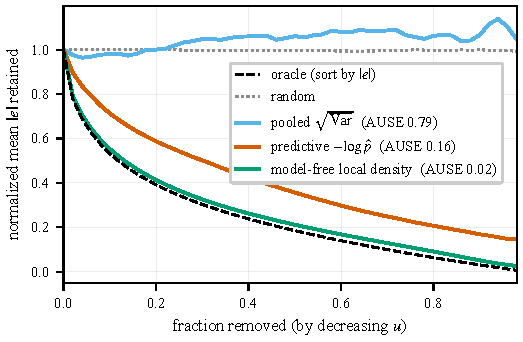
\includegraphics[width=\columnwidth]{figs/mar18_rich_sparsification.pdf}
\caption{Sparsification, March~2018, production configuration
(pipeline product): $200{,}000$ stitched-model samples scored against
the full epoch cloud (Sec.~\ref{sec:setup:metrics}); each curve
removes by its own score (the oracle by $|e|$, random uniformly).
Removing samples by decreasing predictive NLPD
tracks the error oracle far better than random removal (AUSE 0.161,
AURG 0.577); other epochs alike (Table~\ref{tab:coverage}). The
$\sqrt{\overline{\mathrm{Var}}}$ curve is the
location-queryable alternative, nearly uninformative as a ranker
(AUSE 0.786, AURG $-0.05$); the model-free local-density control
(AUSE 0.023, AURG 0.719)
outranks the NLPD ranker and nearly attains the oracle
(Sec.~\ref{sec:results:sparsification}).}
\label{fig:sparsification}
\end{figure}

On the real epochs the ranker is genuinely better than random on
every one (Table~\ref{tab:coverage},
Fig.~\ref{fig:sparsification}; production AUSE 0.161--0.205, AURG
0.521--0.577). The ranking is capacity-\emph{insensitive} (March~2018
AUSE 0.161 at $\hat{K}=841$ versus 0.165 at $\hat{K}=42$), so the
residual oracle gap is not a resolution artifact.

\looseness=-1 The signal decomposes honestly. Predictive uncertainty correlates
strongly with local point density ($\rho(u,\mathrm{density})$ of
$-0.74$, $-0.70$, $-0.67$ at production): sparser regions are genuinely
reconstructed worse, which is causally meaningful but not to be mistaken
for pure model structure.
Density-tercile stratification localizes the residual: within-tercile
AUSE is 0.28--0.50 at production, and the within-tercile gain over
random concentrates in the \emph{sparsest} tercile (AURG 0.19--0.29);
the denser terciles sit essentially at random (AURG $-0.01$ to
$0.03$), so the global ranking's power rides substantially on the
density component. The sparsest-tercile concentration holds at the reference arm as
well, so we attribute the confound to the intrinsic mismatch between
LiDAR point-density heteroscedasticity and the Gaussian likelihood
(Sec.~\ref{sec:disc-density}). For completeness, the alternative
per-point uncertainty $\sqrt{\overline{\mathrm{Var}}}$
of Sec.~\ref{sec:setup:metrics}
is nearly uninformative (AURG $-0.05$ to $+0.14$ across the six runs),
close to piecewise-constant within components. The distinction matters:
$\sqrt{\overline{\mathrm{Var}}}$ is the location-queryable uncertainty; the
predictive NLPD is an a posteriori quality-assurance instrument for
the reconstruction (Sec.~\ref{sec:setup:metrics}), not a
before-measurement error map.

\looseness=-1 The model-free control settles how much of that power is the model's
own: ranking by raw local density of the reference cloud alone
attains AUSE $0.023$--$0.024$ and AURG $0.71$--$0.72$ on the three
epochs, decisively better than the NLPD ranker, and wins within every
density tercile (AUSE $0.07$--$0.16$ vs.\ $0.28$--$0.50$); the two
orderings agree at Spearman $\rho = 0.67$--$0.74$. The NLPD ranking
is thus largely internalized sampling density, its non-density
residual adding no within-tercile power. One caveat runs in the
control's favor: $e$ is the plane distance to the same six neighbors
whose spacing defines the density, so sparse neighborhoods
mechanically inflate $e$ ($\rho$ up to $0.92$), flattering the
control's near-oracle AUSE, though the within-tercile comparison,
which coarsely controls this, still favors density. What the
predictive retains is not ranking power but form: calibrated
intervals and a ${\sim}10^{3}$-component normalized density queryable
without the $10^{7}$-point cloud (Sec.~\ref{sec:disc-density}).

\subsection{Absolute Geometric Accuracy Against the Reference Mesh}
\label{sec:results:geoacc}

\looseness=-1 The sparsification ranker is scored against the same-epoch cloud;
Table~\ref{tab:geoacc} answers the remaining absolute question:
meters against the H3D March~2018 reference mesh, in both directions,
under the protocol of Sec.~\ref{sec:setup:metrics}. Globally the
stitched model reconstructs the surface to mean $0.518$~m (median
$0.267$, RMS $0.863$, P90 $1.32$); completeness reaches $0.665$
within $0.5$~m and $0.951$ within $1$~m (the $0.25$~m fraction,
$0.254$, sits at the $0.326$~m sampling floor and is not
interpretable below it). The choice of seam rule is immaterial at this
scale: crop and Voronoi agree with the stitched model to within
$3$~mm in mean and $1.1$~mm in median in both directions (crop's
accuracy RMS runs $2.6$~cm higher, a tail effect only), consistent
with the parity of Table~\ref{tab:seam}.

\begin{table}[!t]
\caption{Geometric accuracy and completeness (meters) of the
March~2018 production fit against the H3D reference mesh, overall and
stratified by the stitched model's own predictive-NLPD terciles.
Accuracy: $197{,}508$ model samples, exact point-to-mesh distance.
Completeness: $140{,}574$ domain-masked mesh-surface samples to the
nearest of $5\times10^{5}$ model samples (resolution floor
$0.326$~m; the $\le0.25$~m fractions are floor-limited).
Completeness within $1$~m is $0.951$ overall
($1.00$/$1.00$/$0.86$ by tercile). Source:
\texttt{geoacc\_mar18.json}.}
\label{tab:geoacc}
\centering
\setlength{\tabcolsep}{4.5pt}
\begin{tabular}{lrrrrrr}
\hline
 & Mean & Med. & RMS & P90 & $\le$0.25\,m & $\le$0.5\,m \\
\hline
\multicolumn{7}{l}{\emph{Accuracy} (model $\to$ mesh)} \\
All samples & 0.518 & 0.267 & 0.863 & 1.320 & 0.479 & 0.690 \\
\enskip low NLPD  & 0.144 & 0.108 & 0.215 & 0.289 & 0.856 & 0.978 \\
\enskip mid NLPD  & 0.415 & 0.289 & 0.604 & 0.898 & 0.432 & 0.752 \\
\enskip high NLPD & 0.994 & 0.724 & 1.350 & 2.147 & 0.148 & 0.340 \\
\hline
\multicolumn{7}{l}{\emph{Completeness} (mesh $\to$ model)} \\
All samples & 0.452 & 0.380 & 0.547 & 0.821 & 0.254 & 0.665 \\
\enskip low NLPD  & 0.250 & 0.239 & 0.272 & 0.392 & 0.540 & 0.980 \\
\enskip mid NLPD  & 0.402 & 0.387 & 0.435 & 0.624 & 0.182 & 0.739 \\
\enskip high NLPD & 0.704 & 0.655 & 0.796 & 1.092 & 0.041 & 0.276 \\
\hline
\end{tabular}
\end{table}

\begin{figure}[!t]
\centering
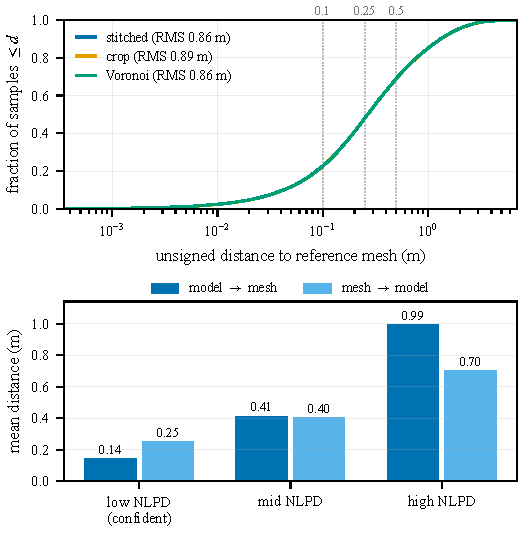
\includegraphics[width=\columnwidth]{figs/geoacc_mar18.pdf}
\caption{Geometric accuracy against the H3D March~2018 reference mesh
(pipeline product). Top: empirical CDF of unsigned model$\to$mesh
distance for the three seam rules (log axis; dotted lines at the
$0.1$/$0.25$/$0.5$~m thresholds): the rules are indistinguishable
(curves overplot to line width).
Bottom: mean distance by the stitched model's own predictive-NLPD
tercile, both directions; the stratification is monotone, and the
confident tercile is decimeter-grade.}
\label{fig:geoacc}
\end{figure}

\looseness=-1 The stratification is the operative finding
(Table~\ref{tab:geoacc}, Fig.~\ref{fig:geoacc}): ordering by the
model's own predictive NLPD (no reference data in the loop)
stratifies the error monotonically in both directions, with accuracy
tercile means of $0.144$/$0.415$/$0.994$~m. The confident third is
decimeter-grade ($85.6\%$ of its samples within $0.25$~m of the mesh,
$97.8\%$ within $0.5$~m), and the model itself identifies it.

\looseness=-1 The honest scope: these are decimeter-to-meter numbers. Classical
photogrammetric--LiDAR survey processing delivers centimeter-grade
products on data of this quality (the reference mesh itself comes
from such a chain), and the meter-band high-NLPD tail is consistent
with the ${\approx}1$~m level-of-detection floor of
Sec.~\ref{sec:results:change} (Sec.~\ref{sec:disc-lod}). What the
stitched density offers is not centimeter accuracy but a calibrated
map that knows where it is good: a self-identified decimeter-grade
core, and meter-band tails the model itself flags.

\subsection{Change Detection with a Model-Derived Level of Detection}
\label{sec:results:change}

% Synthetic slab confirmation: change_synth_slab.json (slab_summary).
The LoD$_{95}$ test of Sec.~\ref{sec:setup:metrics} applied to the
November~2018/March~2019 production fits (Fig.~\ref{fig:change}) takes
21.3~s on the
$313\times783$-cell grid ($113{,}020$ valid cells); on a synthetic 30~cm
displacement slab it attains recall 1.000, null flag rate 0.000, and
$0.06\%$ displacement error, confirming the machinery before any
real-data claim.

\begin{figure}[!t]
\centering
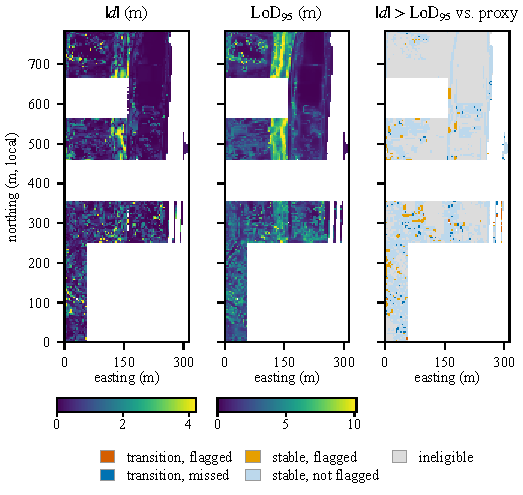
\includegraphics[width=\columnwidth]{figs/change_nov18_mar19.pdf}
\caption{Model-derived change detection, November~2018 vs.\ March~2019
(pipeline product): absolute inter-epoch elevation difference $|d|$,
per-cell LoD$_{95}$, and flagged cells against the class-transition
proxy on the 1~m grid; stable impervious cells calibrate the test
(4.2\% exceedance vs.\ nominal 5\%). White cells (all panels) have
fewer than 20 points in either epoch. Color scales are clipped at the
99th percentile; isolated flagged/transition cells are dilated by one
cell for visibility.}
\label{fig:change}
\end{figure}

\looseness=-1 \emph{Null calibration is delivered.} On the $17{,}592$ physically stable
impervious cells the exceedance rate is 4.2\% against the nominal 5\%
(median $|d|$ 0.17~m; median LoD$_{95}$ 1.16~m), insensitive to the
2~cm registration term (exceedance rate and AUC both shift by
${\sim}10^{-4}$). \emph{Detection is above chance}: on the
vegetation-excluded transition proxy (734 positives, $42{,}487$
negatives), AUC is 0.718 with recall 0.208 and precision 0.081 at the
LoD$_{95}$ threshold on 1~m cells; coarsening to 2~m cells raises AUC to
0.78 and recall to 0.35 with the null still calibrated (4.8\%), while
0.5~m cells give AUC 0.68. Across valid cells median $|d|$ is 0.28~m
(95th pct.\ 2.48~m) vs.\ median LoD$_{95}$ 1.84~m; per the
proxy caveat of Sec.~\ref{sec:setup:protocols}, the false-alarm role
belongs to the null test, not to precision at the threshold.

\begin{table}[!t]
\caption{Change detection on 1~m cells: capacity dose--response of the
model-derived test (both arms at $\sigma_{\mathrm{reg}}=0$;
high-capacity arm: $\alpha=1000$, $T=1024$, $\hat{K}=3443/3525$ for
Mar.~2019/Nov.~2018) beside the classical propagated-error DoD
on identical cells, masks, and proxy (Sec.~\ref{sec:setup:metrics}).
Sources: \texttt{change\{,\_xrich,\_classical\}\_nov18\_mar19.json}.}
\label{tab:change_dose}
\centering
\setlength{\tabcolsep}{3pt}
\begin{tabular}{lcccc}
\hline
 & \multicolumn{2}{c}{Model-derived} &
\multicolumn{2}{c}{Classical DoD} \\
 & Prod. & High cap. & $\sigma_{\mathrm{reg}}{=}0$ &
$\sigma_{\mathrm{reg}}{=}2$\,cm \\
\hline
Null exceedance (nom.\ 5\%) & 4.2\% & 0.9\% & 89.5\% & 17.1\% \\
AUC (veg-excluded)          & 0.718 & 0.776 & 0.816 & 0.973 \\
Precision at LoD$_{95}$     & 0.081 & 0.207 & 0.021 & 0.050 \\
Recall at LoD$_{95}$        & 0.208 & 0.177 & 0.984 & 0.971 \\
Median null-cell LoD$_{95}$ & 1.16~m & 1.04~m & 1.3~mm & 3.9~cm \\
\hline
\end{tabular}
\end{table}

\looseness=-1 The dose--response (Table~\ref{tab:change_dose}) settles whether more
model is the answer. Tripling capacity sharpens the test: precision
at the threshold rises from $0.081$ to $0.207$ and AUC from $0.718$
to $0.776$, at slightly lower recall ($0.177$ vs.\ $0.208$) and a
markedly more conservative null ($0.9\%$ against nominal
5\%). But the LoD floor stays at ${\approx}1.0$~m: a representation
limit (Sec.~\ref{sec:disc-lod}).

\looseness=-1 Table~\ref{tab:change_dose} also delivers the promised classical
yardstick, on literally identical cells. The propagated-error DoD
posts a far sharper nominal threshold (median null-cell LoD$_{95}$
of $1.3$~mm at $\sigma_{\mathrm{reg}}=0$, $3.9$~cm at $2$~cm, against
$1.16$~m) and, as a pure ranking score, separates the transition
proxy better (AUC $0.816$; $0.973$ with the registration term). As a
\emph{detector} it is severely anti-conservative here: $89.5\%$
($17.1\%$ with the registration term) of the stable impervious cells
exceed its nominal-5\% threshold, against $4.2\%$ for the model arm,
because the per-cell standard error shrinks as $1/\sqrt{n}$ (cells
hold hundreds of points) while inter-epoch registration and roughness
error do not. The model-derived LoD is thus deliberately
conservative (recall $0.21$ against $0.97$, with a held null) and
offers what the DoD cannot: the uncertainty rides in the fitted
mixtures, so calibrated change maps need no per-cell access to both
epochs' raw clouds at comparison time.

\subsection{Variance-Guided Re-Flight Planning}
\label{sec:results:reflight}

On the Mill~19 Rubble anchor (Sec.~\ref{sec:setup:protocols};
$1.75\times10^{6}$ points, 1{,}678 images) the re-flight experiment
asks whether the model's own posterior can plan the next flight; all
arms are scored on one frozen evaluation set that no refit ever sees
(Table~\ref{tab:reflight}). The null control frames the block
scenarios: with held-back imagery \emph{interleaved} through the
survey, no planner, including the error oracle, moved held-out NLPD
by more than $0.04$~nats at a 20\% or 50\% dose: re-flying covered
ground buys nothing; the operational case is contiguous \emph{new}
ground.

\begin{table}[!t]
\caption{Re-flight planning on Mill~19 Rubble (block holdback, new
ground): improvement in mean held-out NLPD (nats; baseline $-$ arm),
overall and within the granted tiles. Random arms: mean $\pm$ sample
s.d.\ over seeded replicates. $^{\dagger}$Selects the same tiles
as expected yield, so the rows coincide.
$^{\ddagger}$Selects the same tiles as the error oracle (row
omitted as a duplicate). Sources:
\texttt{reflight\_rubble\_*\_v2.json},
\texttt{reflight\_rubble\_mass\{6,12\}.json}.}
\label{tab:reflight}
\centering
\setlength{\tabcolsep}{4pt}
\begin{tabular}{llrr}
\hline
Scenario & Planner & $\Delta$ overall & $\Delta$ granted \\
\hline
Block, 6 tiles    & uncertainty$^{\ddagger}$ & $+1.10$ & $+1.90$ \\
(2 grants)        & mass only          & $+0.86$ & $+1.37$ \\
                  & random (5 seeds)   & $+0.45 \pm 0.17$ & $+1.45 \pm 0.54$ \\
\hline
Block, 12 tiles   & raw NLPD ranking   & $+0.14$ & $+1.88$ \\
(3 grants)        & expected yield     & $+1.15$ & $+1.45$ \\
                  & mass only$^{\dagger}$ & $+1.15$ & $+1.45$ \\
                  & error oracle       & $+0.55$ & $+1.96$ \\
                  & random (8 seeds)   & $+0.46 \pm 0.42$ & $+1.15 \pm 0.52$ \\
\hline
\end{tabular}
\end{table}

\looseness=-1 \emph{Act 1: posterior uncertainty finds where the model is wrong.} On
the 6-tile site grid, with the unfinished 20\% strip held back, the
uncertainty
planner selects exactly the tiles the error oracle selects and
improves held-out NLPD by $+1.10$~nats, above every random grant
($+0.45\pm0.17$, 5 seeds; best $+0.61$); the gain is local, not drift
($+1.90$ inside the granted tiles). It also beats the mass-only
control, which grants 8\% more points ($128{,}344$ vs.\ $118{,}730$)
yet achieves only $+0.86$: the posterior finds \emph{which}
comparable-mass ground is badly modeled, not merely \emph{where} data
are recoverable.

\looseness=-1 \emph{Act 2: raw uncertainty is mass-blind.} On the finer 12-tile grid,
ranking tiles by raw mean NLPD still targets genuinely bad tiles
($+1.88$ inside its grants) but selects tiles with almost no
recoverable imagery: it grants only $19{,}734$ pool points and moves
the overall score by $+0.14$, below the random mean of
$+0.46\pm0.42$ (seed range $+0.00$ to $+0.99$).

\looseness=-1 \emph{Act 3: where mass separates tiles, mass dominates.} Scoring tiles by \emph{expected yield} (mean tile NLPD $\times$
grantable pool mass; the NLPD factor is available before flying, while
the mass factor, measured here from the held-back block, stands in for
the coverage-based yield estimate a planner would form in advance)
resolves the failure:
$+1.15$~nats held-out (Table~\ref{tab:reflight}), above all eight
random draws (best $+0.99$), and raises the fraction of evaluation
points within $0.5$~m of a model sample by $+0.09$. But so does recoverable mass alone: the mass-only control
selects the identical tiles and matches $+1.15$ exactly. On this grid
the posterior factor adds no selection signal, and the margin over
the error oracle (itself at $+0.55$) is carried by the mass term: the oracle's
grants carry $62{,}387$ pool points against the yield planner's
$157{,}739$. Read together with Act~1: mass is the first-order
planning signal, and the posterior's measured value concentrates
exactly where mass stops discriminating.
